%% LyX 2.4.4 created this file.  For more info, see https://www.lyx.org/.
%% Do not edit unless you really know what you are doing.
\documentclass[english]{article}
\usepackage[T1]{fontenc}
\usepackage[latin9]{inputenc}

\makeatletter
%%%%%%%%%%%%%%%%%%%%%%%%%%%%%% User specified LaTeX commands.

%%%%Tree%%%%
%\usepackage[latin1]{inputenc}
\usepackage{tikz}
\usetikzlibrary{trees}
%%%%Scenario%%%%%
%\usepackage{tikz} 
\usepackage{verbatim}
\usetikzlibrary{shapes} 
\usepackage{amsmath} 
\usepackage{xspace} 

\makeatother

\usepackage{babel}
\begin{document}

\section{Tree Diagrams}

%%Simple Tree Diagram%%%%
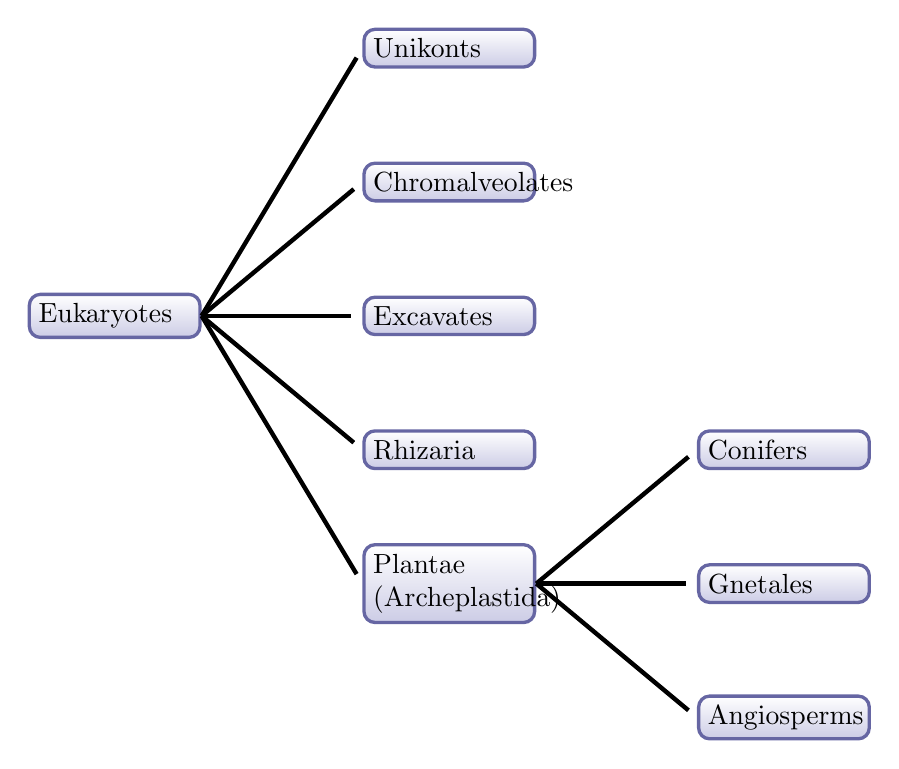
\begin{tikzpicture}
	[scale=.85,
		every node/.style = {rectangle, rounded corners, shade, top color=white,     bottom color=blue!50!black!20, draw=blue!40!black!60, very     thick, text width=5.5em},                    
	blue edge/.style  = {-,ultra thick,black,shorten >= 4pt}
	]
% the nodes : possible  \newcommand*\dx{5} \newcommand*\dy{2} 
\node(0;0) at (0,0) {Eukaryotes};   
	\node(1;2)  at (5, 4) {Unikonts};      
	\node(1;1)  at (5, 2) {Chromalveolates};    
	\node(1;0)  at (5, 0) {Excavates};    
	\node(1;-1) at (5,-2) {Rhizaria};    
	\node(1;-2) at (5,-4) {Plantae\\(Archeplastida)};      
		\node(2;1)  at (10,-2) {Conifers};      
		\node(2;0)  at (10,-4) {Gnetales};      
		\node(2;-1) at (10,-6) {Angiosperms};
% edges  
	\foreach \j in {-2,...,2}   { \draw[blue edge] (0;0.east) -- (1;\j.west);} 
	\foreach \j in {-1,...,1}  { \draw[blue edge] (1;-2.east) -- (2;\j.west);}                   
\end{tikzpicture}

% Set the overall layout of the tree 
\tikzstyle{level 1}=[level distance=3.5cm, sibling distance=3.5cm] 
\tikzstyle{level 2}=[level distance=3.5cm, sibling distance=2cm]

% Define styles for bags and leafs 
\tikzstyle{bag} = [text width=4em, text centered] 
\tikzstyle{end} = [circle, minimum width=3pt,fill, inner sep=0pt]

% The sloped option gives rotated edge labels. Personally 
% I find sloped labels a bit difficult to read. Remove the sloped options 
% to get horizontal labels.  

\begin{tikzpicture}[grow=right, sloped] 
\node[bag] {Bag 1 $4W, 3B$}     
	child {
		node[bag] {Bag 2 $4W, 5B$}                    	   	
			child {node[end, label=right: 
				{$formulas$}] {}               			
				edge from parent                 
					node[above] {$W$}                 			
					node[below]  {$\frac{4}{9}$}             
			}             	
			child {node[end, label=right:                     			
					{$formauls$}] {}                 
					edge from parent                 				
						node[above] {$B$}                 				
						node[below]  {$\frac{5}{9}$}             		
			}             
			edge from parent              			
				node[above] {$W$}             			
				node[below]  {$\frac{4}{7}$}     
	}     
	child {         
		node[bag] {Bag 2 $3W, 6B$}                 							
			child {node[end, label=right:                     			
					{$Pformulas$}] {}                 
					edge from parent                 			
						node[above] {$B$}                 					
						node[below]  {$\frac{3}{9}$}             		
			}             
			child {node[end, label=right:
					{$formulas$}] {}                 
					edge from parent                 			
						node[above] {$W$}                 			
						node[below]  {$\frac{6}{9}$}             		
			}         
	edge from parent                      		
		node[above] {$B$}             
		node[below] {$\frac{3}{7}$}     
	}; 
\end{tikzpicture} 

% Scenario tree 
% Author: Rasmus Pank Roulund \documentclass{minimal} 

\newcommand{\A}{\ensuremath{\mathcal{A}}\xspace} 
\newcommand{\B}{\ensuremath{\mathcal{B}}\xspace} 
\newcommand\pa[1]{\ensuremath{\left(#1\right)}} 

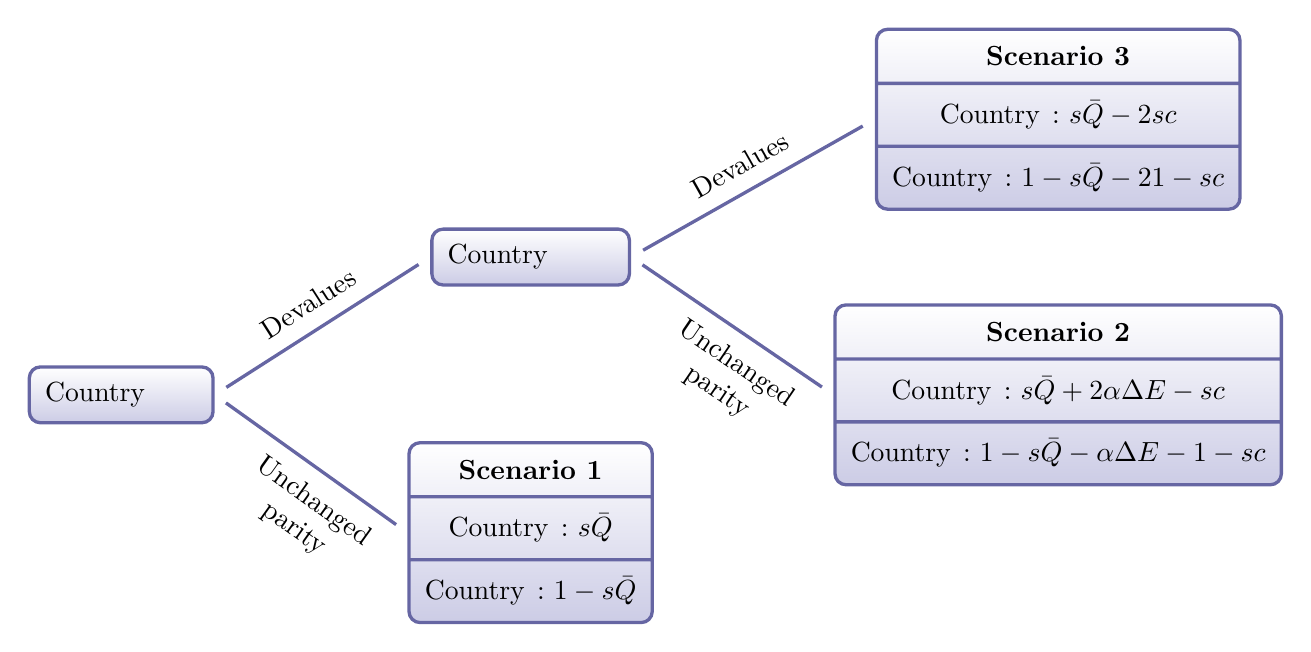
\begin{tikzpicture}[grow=right,     
	level 1/.style={
		sibling distance=3.5cm,
		level distance=5.2cm},     
	level 2/.style={
		sibling distance=3.5cm, 
		level distance=6.7cm},     
	edge from parent/.style={
		very thick,draw=blue!40!black!60,         
		shorten >=5pt, shorten <=5pt},     
	edge from parent path=
		{(\tikzparentnode.east) -- (\tikzchildnode.west)},     
	kant/.style={text width=2cm, 
		text centered, sloped},     
	every node/.style={text ragged, inner sep=2mm},     
	punkt/.style={rectangle, rounded corners, 
		shade, top color=white,     
		bottom color=blue!50!black!20, 
		draw=blue!40!black!60, 
		very     thick }     
	]

\node[punkt, text width=5.5em] {Country~\B}     
	%Lower part lv1     
	child {node[punkt] 
		[rectangle split, 
		rectangle split, 
		rectangle split parts=3,          
		text ragged] 
		{\textbf{Scenario  1}                   
		\nodepart{second}             
			$\text{Country \B}\colon    s\bar{Q}$                   
		\nodepart{third}             
			$\text{Country \A}\colon\pa{1-s}\bar{Q}$  
		}         
	edge from parent             
		node[kant, below, pos=.6] {Unchanged parity}     
	}     
	%Upper part, lv1     
	child {node[punkt, text width=6em] {Country~\A}         
		%child 1         
		child {node [punkt,
					rectangle split, 
					rectangle split,             
					rectangle split parts=3] 
			{\textbf{Scenario  2}                 
				\nodepart{second}
					$\text{Country \B}\colon s\bar{Q}+2\alpha\Delta E -sc$                 				\nodepart{third}                 
					$\text{Country \A}\colon\pa{1-s}\bar{Q}-\alpha\Delta E - \pa{1-s}c$             
		}            
		edge from parent                 
			node[below, kant,  pos=.6] {Unchanged parity}         
	}         
		%child 2         
		child {node [punkt, 
				rectangle split, 
				rectangle split parts=3]
					{\textbf{Scenario 3}                 
				\nodepart{second}                 
					$\text{Country \B}\colon s\bar{Q}-2sc$                 
				\nodepart{third} 
					$\text{Country \A}\colon\pa{1-s}\bar{Q}-2\pa{1-s}c$             
		}             
		edge from parent                 
			node[kant, above] {Devalues}}             
		edge from parent{
			node[kant, above] {Devalues}}     
	}; 
\end{tikzpicture} 
\end{document}
